\chapter{Descrierea aplicației AudIT}
Adaptarea la noile paradigme tehnologice ne impune tuturor o provocare, mai mult sau mai puțin dificilă , instituțiile publice ale statului confruntându-se zilnic cu această problemă, este nevoie cât mai repede de o soluție eficientă care va rezolva aceasta problemă.

\par Prima secțiune a acestei lucrări urmăreste să exploreze în detaliu cum platforma AudIT se aliniază și contribuie la acțiunea de transformare și adaptare digitală în sectorul public, analizând componentele cheie ale aplicației în raport cu problemele pe care aceastea incearcă sa le rezolve.


\section{Problema adresată}
Digitalizarea, potrivit definiției este procesul de transformare a informațiilor dintr-un format analogic, hârtii, într-un format digital, biți. De fapt, acest procedeu constituie o adevarată nouă paradigma în materie de algoritmi administrativi, sensul de derulare al întregului sistem și metodele utilizate de către factorul uman în dezvoltarea soluțiilor.
\par În decursul discutiilor  cu tatăl meu, auditor public, au fost descoperite numeroase 
puncte nevralgice în metodele și soluțiile folosite de auditorii publici din România pentru a duce la capăt anumite întrebuințări de serviciu. Acestea pot părea nesemnificative pe moment, dar observând fenomenul la scară largă, de exemplu,  pe întreg parcurul unei misiuni de audit public, care poate dura pana la câteva luni, constatăm faptul că intreg procesul și eficiența auditorului sunt major încetinite de aceste imperfecțiuni.

\par Una dintre cele mai mari probleme prezente in procesul de audit public, și cel mai probabil în majoritatea instituțiilor publice din tară, este nevoia de a folosi și a administra inventarul a multor documente oficiale, pierzând astfel mult timp în identificarea documentului corespunzător acțiunii sau activitații pe care auditorul vrea să o efectueaze, ulterior pierzând și mai mult timp în completarea și în comunicarea și transmiterea acestui act către reprezentantul agenției sau departamentului auditat. De acest lucru este strâns legată și problema comunicării între parțile care participă la misiunea de audit public, aceasta realizându-se în majoritatea cazurilor prin intermediul poștei iar uneori dacă distanța permite chiar prin intermediul unor 'curieri umani'. 

\par  Având în vedere aceste \textit{vulnerabilități} din sistemul public de audit, platforma web AudIT a fost concepută pentru a răspunde nevoii de adaptare și transformare digitală, încercând în același timp să îmbunatațească protocoalele și procesele interne, astfel permitând factorului uman să își îndeplinească sarcinile într-un mod mult mai ușor și rapid.

\section{Soluția propusă}
Platforma Web AudIT este concepută ca o soluție inovatoare asupra provocărilor datorate digitalizării în instituțiile publice, oferind un set de instrumente și funcționalități care fac mult mai accesibilă și fluentă  munca auditorului public cât și cea a reprezentanților instituțiilor audidate.

\par Aplicația are ca și scop principal creșterea eficienței în procesul de audit public, prin implementarea diferitelor functionalități care vor imbunatati drastic accesul utilizatorilor la informații și documente relevante, vor crește nivelul eficienței, auditorii concentrându-se pe aspectele esențiale ale auditului, fără a-și consuma  astfel timpul și energia pe numeroase sarcini care se pot dovedi repetitive, amănunțite si obositoare în final respectiv va facilita un mod de comunicare eficace între persoanele care iau parte la misiunea de audit.



\section{Functionalitățile aplicatiei}
Subsecțiunile care vor urma o să prezinte în detaliu functionalitățile de bază ale platformei,
modul în care acestea au fost implemnentate, cât și dificultăți și provocări ulterioare în ceea ce privește facilitățile oferite de acestea.

\subsection{Autentificarea pe platformă}
Prima interacțiune a fiecărui utilizator cu platforma web o constituie pagina de autentificare, care asigură faptul că accesul la funcționalitățile aplicației este restricționat doar celor care dețin sau doresc să își creeze un cont pe această aplicație.

Procesul de creare a unui cont nou este conceput astfel încât să se ajusteze pe necesitățile de securitate de bază ale instituțiilor publice.
\par  Presupunând faptul că fiecare angajat al unui departamant dintr-o instituție a statului deține o adresă de email cu domeniul instituției de care aparține, tot ce treuie să facă noul potențial utilizator este să se folosească de această adresă de email ca să își creeze un cont nou. Contul nou este creat cu drepturi limitate, acesta neavând acces la nici o resursă care aparține de instituția sa până în momentul când un reprezentant al instituției nu îi validează contul.
 
 	\vspace{0.5 cm}
 \begin{figure}[h]
 	\centering
 	
 	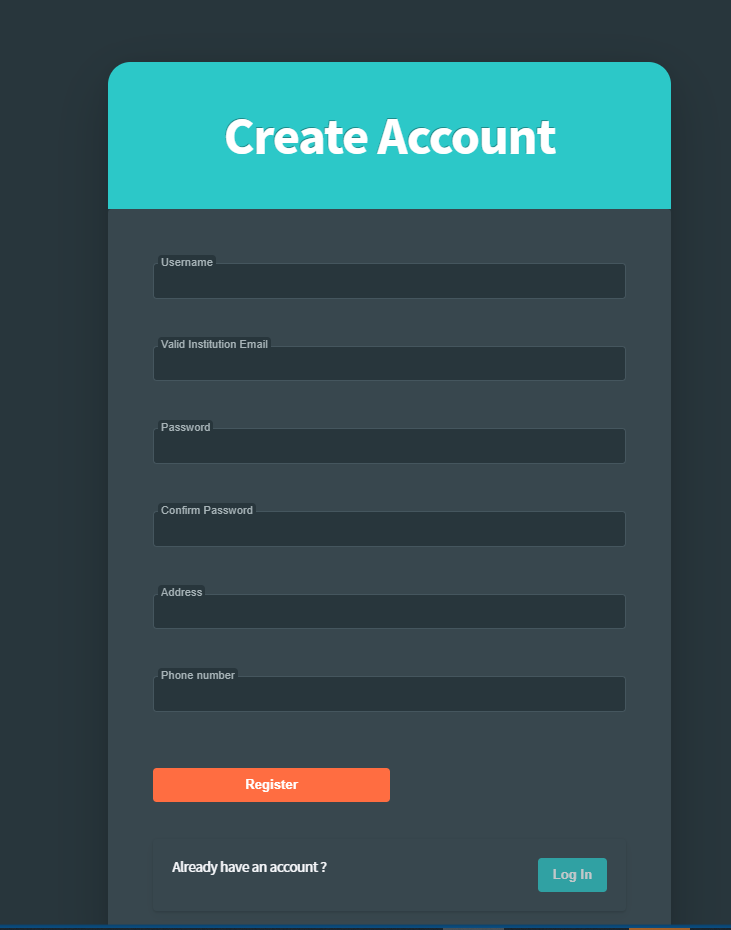
\includegraphics[width=0.5\textwidth]{c1/register.png}
 	\caption{Înregistrarea  pe platformă}
 \end{figure}
 
Această metodă de autentificare se bazează pe o  configurare inițială a unor utilizatori cu drepturi elevate, reprezentanții departamentelor, cărora li se oferă capacitatea de a verifica noii utilizatori care se inregistrează pe platforma utilizând domeniul departamentului în cauză. Fiind pe o parte un mod in plus prin care se limitează accesul utilizatorilor la anumite resurse până când identitatea acestora este confirmată, este pe de altă parte un pas necesar care nu prezintă momentan un sistem de automatizare a verificării identității utilizatorilor, eliminând astfel nevoia unei configurări inițiale a platformei.
	\vspace{0.5 cm}
\begin{figure}[h]
	\centering
	
	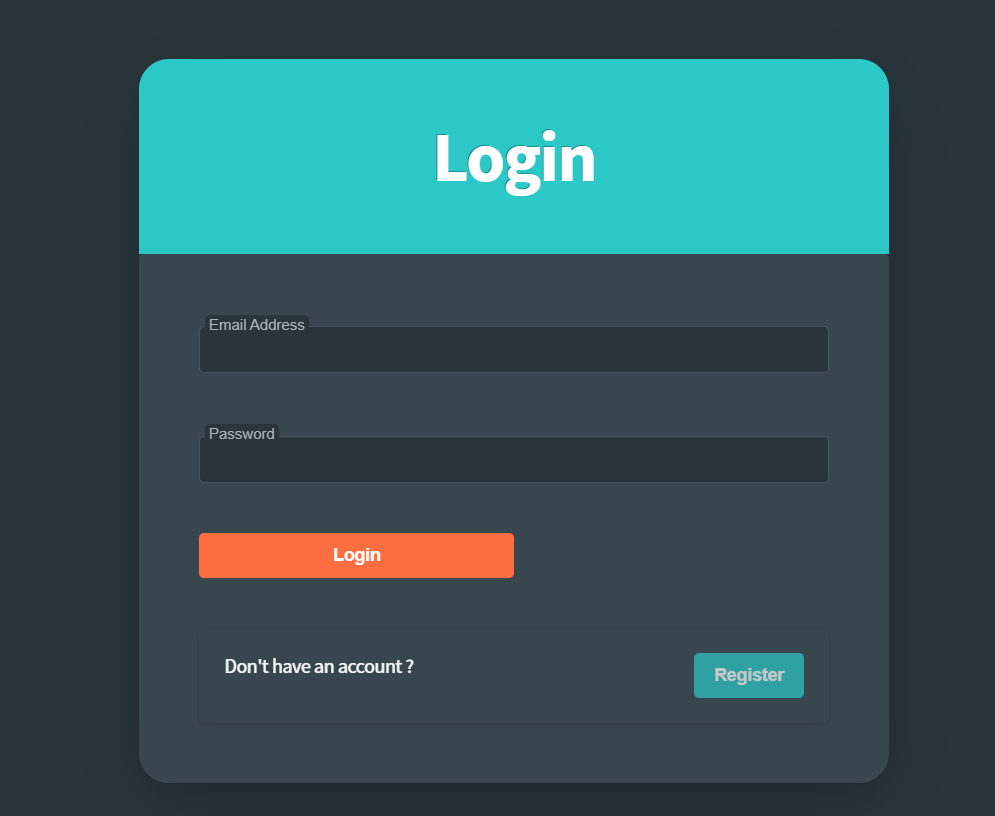
\includegraphics[width=0.5\textwidth]{c1/login.png}
	\caption{Autentificarea pe platformă}
\end{figure}

\subsection{Verificarea acțiunilor utilizatorilor}
În cadrul aplicației, accesul la fiecare entitate este protejat prin implementarea unor liste de acces care definesc permisiunile de scriere și de citire asupra respectivei entități. Acest lucru se asigură că inițial, fiecare utilizator are drept de scriere și de citire doar asupra resurselor create de acesta pe platformă, ulterior acesta având posibilitatea de a acorda sau a primi acces de scriere sau citire asupra altor resurse aflate pe platformă.
	
De asemenea, este implementat și un sistem de roluri care restrictionează și acestea la rândul lor accesul la diferite functionalități ale aplicației, spre exemplu, un utilizator cu rol de reprezentant al unei instituții nu va putea accesa paginile referitoare la crearea sau editarea unei misini de audit.
În plus, pentru o conformitate si pentru o evidență sporită asupra acțiunilor utilizatorilor asupra resurselor de pe platformă este implementat un sistem de auditare al entităților, toate operațiile de creare, modificare și ștergere fiind salvate.

\subsection{Pagina de start}
Pagina de start este locul implicit unde un utilizator este redirecționat atunci când autentificarea sa pe aplicație este cu succes. Aceasta îi prezintă auditorului ultimele modificări la resursele la care are acces, o listă de notificări pe care acesta le-a primit din partea reprezentanților instituțiilor la care auditorul are misiuni de audit în desfășurare cât și diferite butoane de navigare către pagini cheie din aplicație, astfel oferind o interacțiune mai usoară pe platforma AudIT.

\subsection{Gestionarea misinilor de audit public}
În cadrul procesului de audit public, o gestionare eficientă a misiunilor, atât curente cât și din trecut, este esențială pentru o experiență cat mai naturală și intuitivă a utilizatorului pe platformă.

Crearea unei noi misiuni de audit este similară cu crearea unui nou proiect, auditorul specificând numele noii misiuni de audit, instituția respectiv departamentul asupra căruia se realizează noua misiune de audit.

	\vspace{0.5 cm}
\begin{figure}[h]
	\centering
	\begin{minipage}{.5\textwidth}
		\centering
		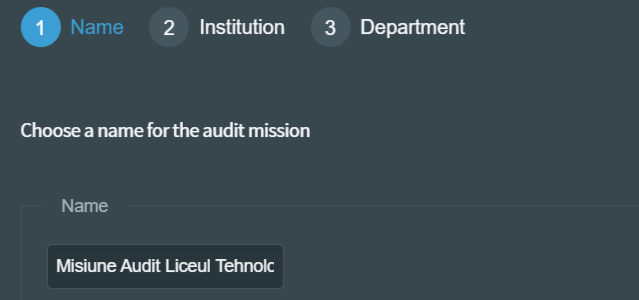
\includegraphics[width=.9\linewidth]{c1/pas1_creare_misiune.png}
		\caption{Stabilirea numelui}
		
	\end{minipage}%
	\begin{minipage}{.5\textwidth}
		\centering
		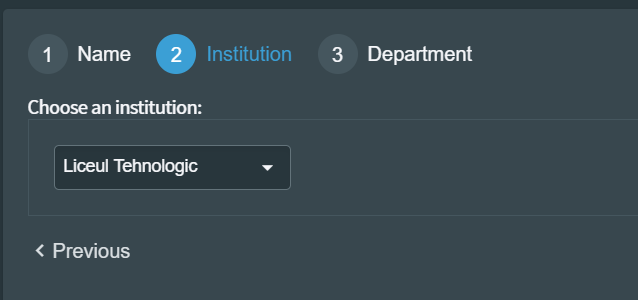
\includegraphics[width=.9\linewidth]{c1/pas2_creare_misiune.png}
		\caption{Selectarea instituției}
	
	\end{minipage}
	\vspace{0.5 cm}

	\centering
	
	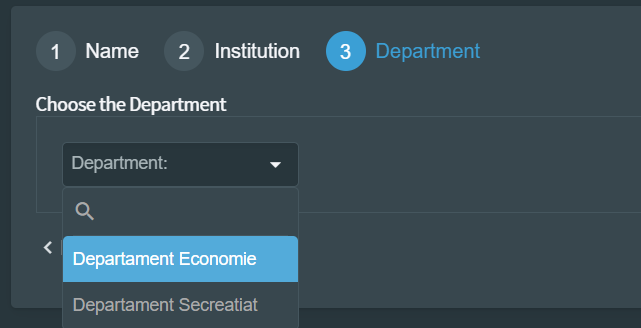
\includegraphics[width=0.5\textwidth]{c1/pas3_creare_misiune.png}
		\vspace{0.5 cm}
	\caption{Selectarea departamentului}
	
	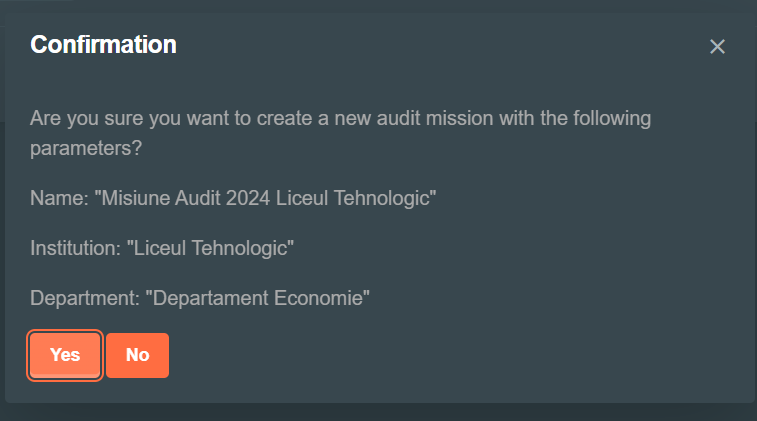
\includegraphics[width=0.5\textwidth]{c1/confirmare_misiune_creata.png}
	\caption{Confirmare creare misiune de audit}
	
\end{figure}


După crearea noii misiuni, auditorul este redirecționat către o pagină în care acesta poate vizualiza intr-un tabel toate misiunile de audit la care acesta are acces, cele create de el, dar și cele la care i-a fost oferit accesul. Afișarea intărilor din tabel este una de tip paginată cu un număr de șapte misiuni pe pagină, astfel încât atenția utilizatorului să fie concentrată doar pe aceste misiuni, în acest fel eliminând posibilitatea de a nu găsi informația pe care acesta o caută datorită unui număr prea mare de linii si informații.
	\vspace{0.5 cm}
\begin{figure}[h]
	\centering
	
	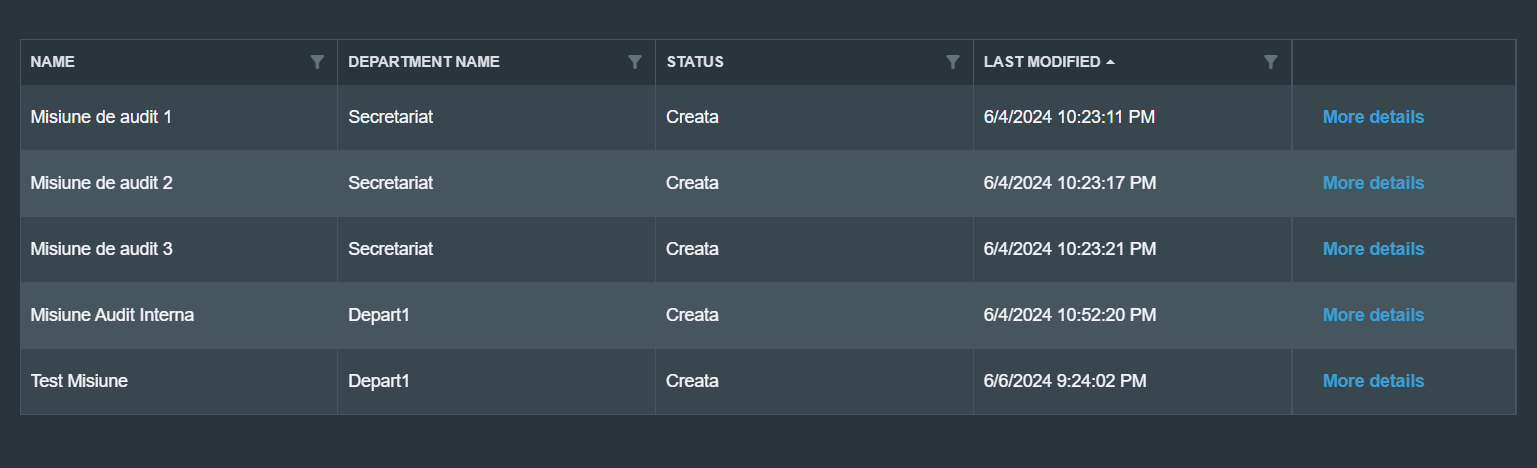
\includegraphics[width=0.8\textwidth]{c1/audit_missions_list.png}
	\caption{Vizualizarea misiunilor de audit}
\end{figure}

De asemenea, informațiile afișate în acest tabel pot fi sortate alfabetic după numele misiunii de audit, după starea în care fiecare dintre acestea se află, după departamentul asupra căruia se desfasoară misiunea  sau după data ultimei modificări a acesteia.

\subsection{Pagina rezumat misiune de audit}

Pagina de rezumat a unei misiuni de audit are ca scop informarea auditorului asupra unei viziuni de ansamblu asupra misiunii de audit respective. Aceasta conține următoarele informații:\\
\begin{itemize}
	
	\item în partea de sus a paginii, auditorului îi este prezentat sub forma unei secvențe de pasi, statusul curent al misiunii, acesta fiind primul lucru pe care privirea utilizatorului il vede;
		
		\begin{figure}[h]
		\centering
		
		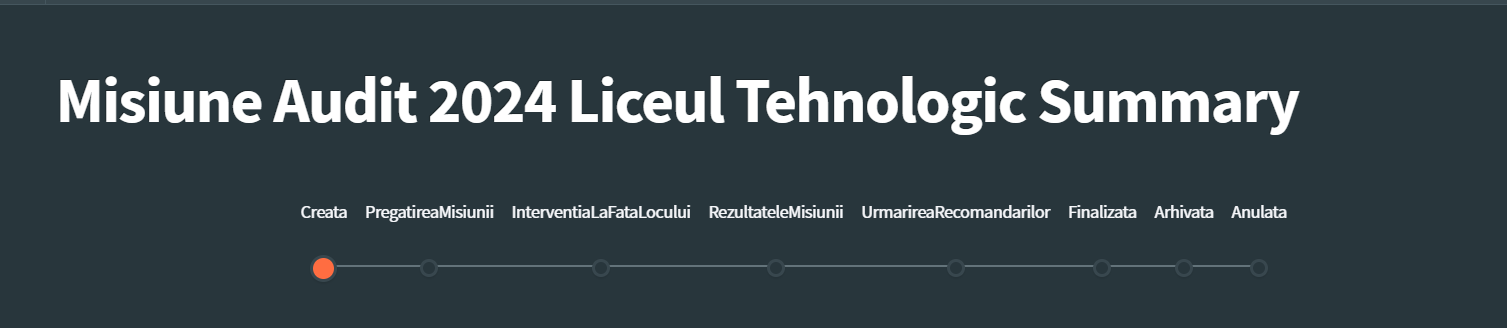
\includegraphics[width=0.9\textwidth]{c1/lant_summary.png}
		\caption{Informații despre statusul misiunii de audit}
	\end{figure}

	\item o scurtă descriere asupra parametrilor misiunii de audit,cum ar fi nume, data ultimii modificări, numele departamentului dar și statusul actual al misiunii. Utilizatorul are opțiunea de a edita acești parametri și a salva modificările aduse;
	
		\vspace{0.5 cm}
	\begin{figure}[h]
		\centering
		
		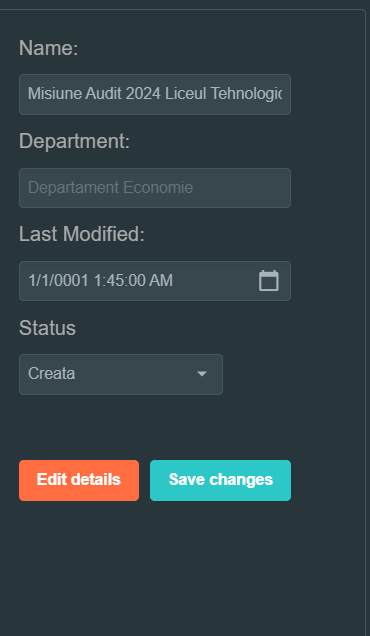
\includegraphics[width=0.5\textwidth]{c1/status_misiune}
		\caption{Informații sumare despre misiunea de audit}
	\end{figure}
	
	\item în partea dreaptă a paginii sunt prezente patru chenare care prezintă cele mai recente modificări și actualizări în materie de : obiective, documente atașate misiunii, fișe de identificare a problemei cât și activități recente asociate misiunii de audit. Utilizatorul are posibilitatea de a naviga apăsând pe numele intrării din lista către pagina dedicată acesteia, sau la apăsarea butonului de 'See more' să fie redirecționat către pagina dedicată tututor entităților de acel fel;
	
	\begin{figure}[h]
		\centering
		
		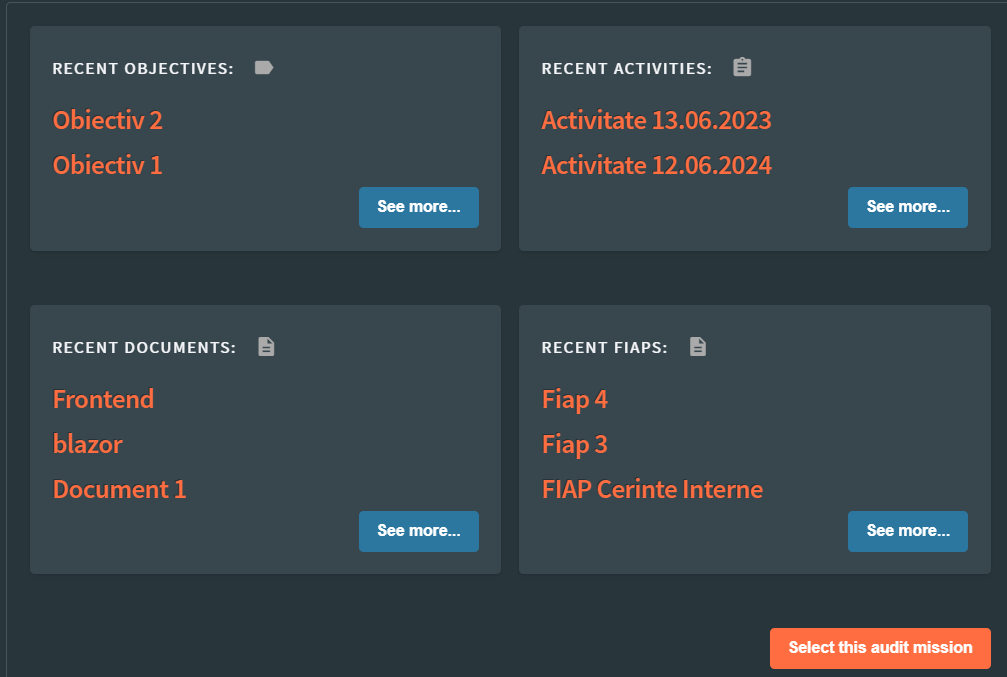
\includegraphics[width=0.7\textwidth]{c1/chenar_recent}
		\caption{Informații sumare despre modificarile recente}
	\end{figure}

	\item în partea dreaptă jos, auditorul are posibilitatea de a selecta misiunea de audit ca fiind misiunea curentă, astfel orice acțiune pe care acesta o sa o facă pe platformă o să ia ca opțiune preselectată misiunea aleasă de acesta.\\
		
	
\end{itemize}


\subsection{Prelucarea pașilor unei misiuni de audit}

Pentru o reproducere cât mai precisă și cooerentă a stagiilor prin care o misiune de audit trece, platforma permite setarea unui status al fiecărei misiuni de audit, astfel auditorul având posibilitatea de a-și marca în detaliu progresul până la momentul curent asupra misiunii de audit. De asemenea, fiecare pas major dintr-o misiune de audit prezintă funcționalități specifice, care vor fi explicate sumar in această subsecțiune.

\subsection*{Pregătirea misiunii de audit}

Pregătirea misiunii de audit este etapa inițială în care auditorul creează misiunea, consultă misiunile anterioare efectuate la același departament, se elaborează un plan de audit, se stabilesc obiectivele, acțiunile specifice fiecărui obiectiv respectiv riscurile specifice fiecărei acțiuni și se întocmesc o serie de documente oficiale, pentru a ține evidența activităților ulterioare pe care auditorul le va realiza în această misiune de audit.

\subsection*{Intervenția la fata locului}

Intervenția la fața locului este o etapă importantă a procesului de audit public, etapă care implică de cele mai multe ori o deplasare in teren unde auditorul efectuează interviuri, realizează eșantioane, analizează riscurile si obiectivele stabilite la pasul anterior și încearcă să înțeleagă într-un mod cât mai corect și obiectiv activitățile desfășurate de departamentul respectiv. Acest pas constă în esență în crearea și completarea a multor documente de tip șablon pe care auditorul le va folosi ulterior în pașii ce urmează pentru a întocmi un raport final.

\subsection*{Rezultatele Misiunii}
După finalizarea pasului anterior, auditorul acum dispune de întreg instrumentalul pentru a întocmi un raport final. Acesta este întocmit pe baza diferitelor întâlniri între auditor și repezentantul instituției, în care se discută aspecte legate de constatările făcute în respectiva misiune de audit. Raportul final cuprinde constatările făcute, recomanandări sub forma 
unor Fișe de Identificare și Analiză a Problemei respectiv cauze și consecințe ale problemelor detectate.

Acest raport este prezentat părților particpante la misiune pentru a le informa asupra rezultatelor misiunii de audit și pentru a ajunge la o înțelegere asupra termenilor de remediere a problemelor pe care aceștia trebuie să le rezolve.

\subsection*{Urmarirea recomandarilor}

Urmărirea recomandărilor este pasul final dintr-o misine de audit în care sunt monitorizate recomandările oferite de către auditor și respectarea termenilor limită de implementare a acestora. Reprezentanții instituțiilor trebuie să ia la cunoștință aceste recomandari și să gasească, ajutați de Fișa de Identificare și Analiză a Problemei corespunzătoare fiecărei recomandari, soluții pentru fiecare chestiune în parte respectând totodată și termenul limită impus de aceasta.


\subsection{Stabilirea obiectivelor de auditat}

Stabilirea obiectivelor de auditat are loc in faza initiala a pasului pregatirii misiunii de audit, pas in care auditorul stabileste obiectivele principale care vor fi auditate in cele ce urmeaza. Fiecare obiectiv este compus din mai multe actiuni specifice iar acestea contin la randul lor o serie de riscuri identificate. Aceste riscuri identificate de catre auditor sunt ierarhizate pe baza unei formule de calcul care ia in considerare probabilitatea actiunii de a se intampla, impactul pe care aceasta il va avea si riscul final rezultat al inmultirii celor doua.

Platforma web AudIT ofera aceste functionalitati utilizatorului, astfel incat acesta sa respecte in detaliu toti pasii legislativi ai procedurii de audit public. Auditorul poate forma obiective noi si sa le ataseze la misiunea de audit corespunzatoare.\\

\begin{figure}[h]
	\centering
	
	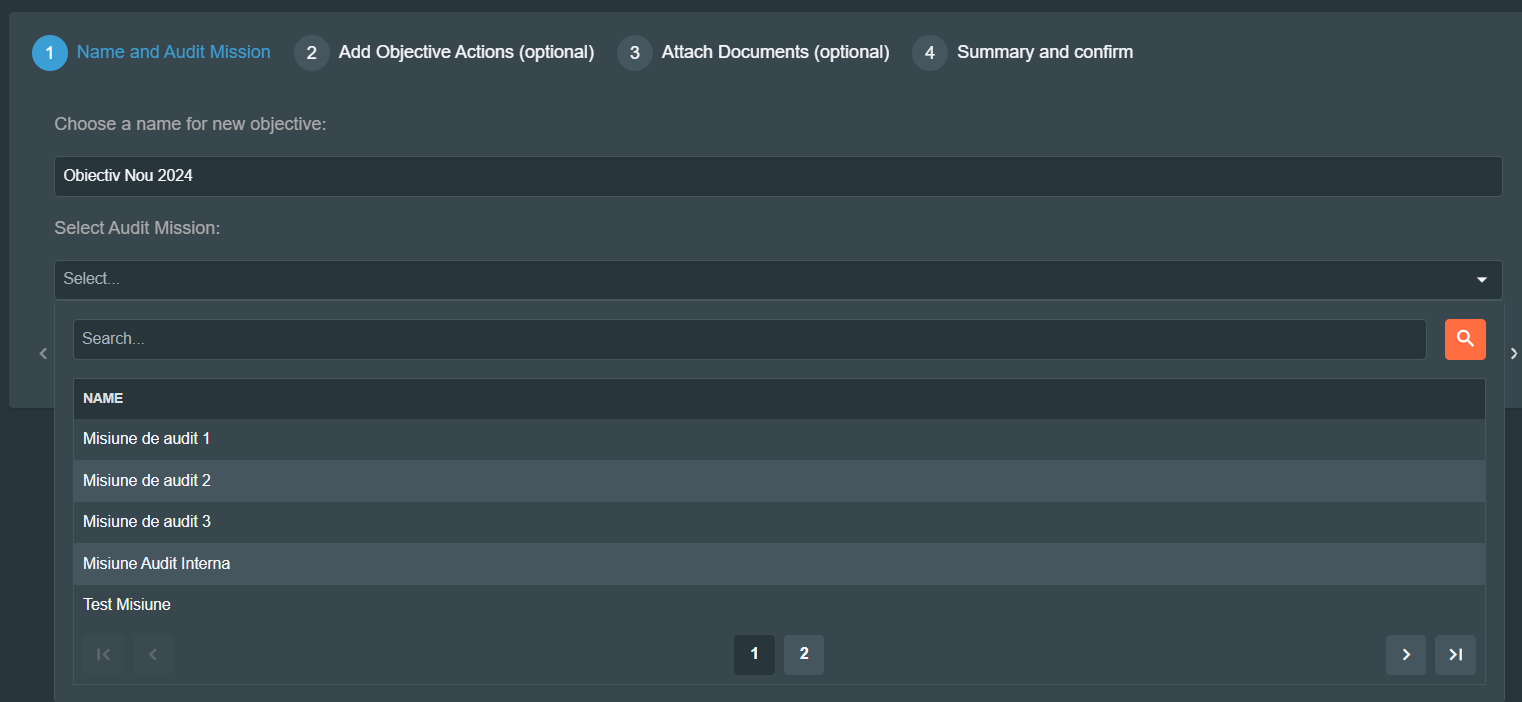
\includegraphics[width=0.8\textwidth]{c1/creare_obiectiv_1}
	\caption{Primul pas in crearea unui nou obiectiv	}
\end{figure}

De asemenea, acesta are posibiliatea de a atasa direct din meniul de creare al unui obiectiv, actiuni specifice obiectibului respectiv, precum si documente necesare sau ajutatore actiunii, astfel usurand semnificativ procesul de inventariere prezent la acest pas.\\
Tot acest proces  de creare a unui nou obiectiv este impartit pe mai multi pasi, astfel incat interactiunea utilizatorului cu aplicatia respectiv cu interfata grafica a acesteia sa fie una cat mai naturala si intuitiva.
\vspace{1cm}
\begin{figure}[h]
	\centering
	
	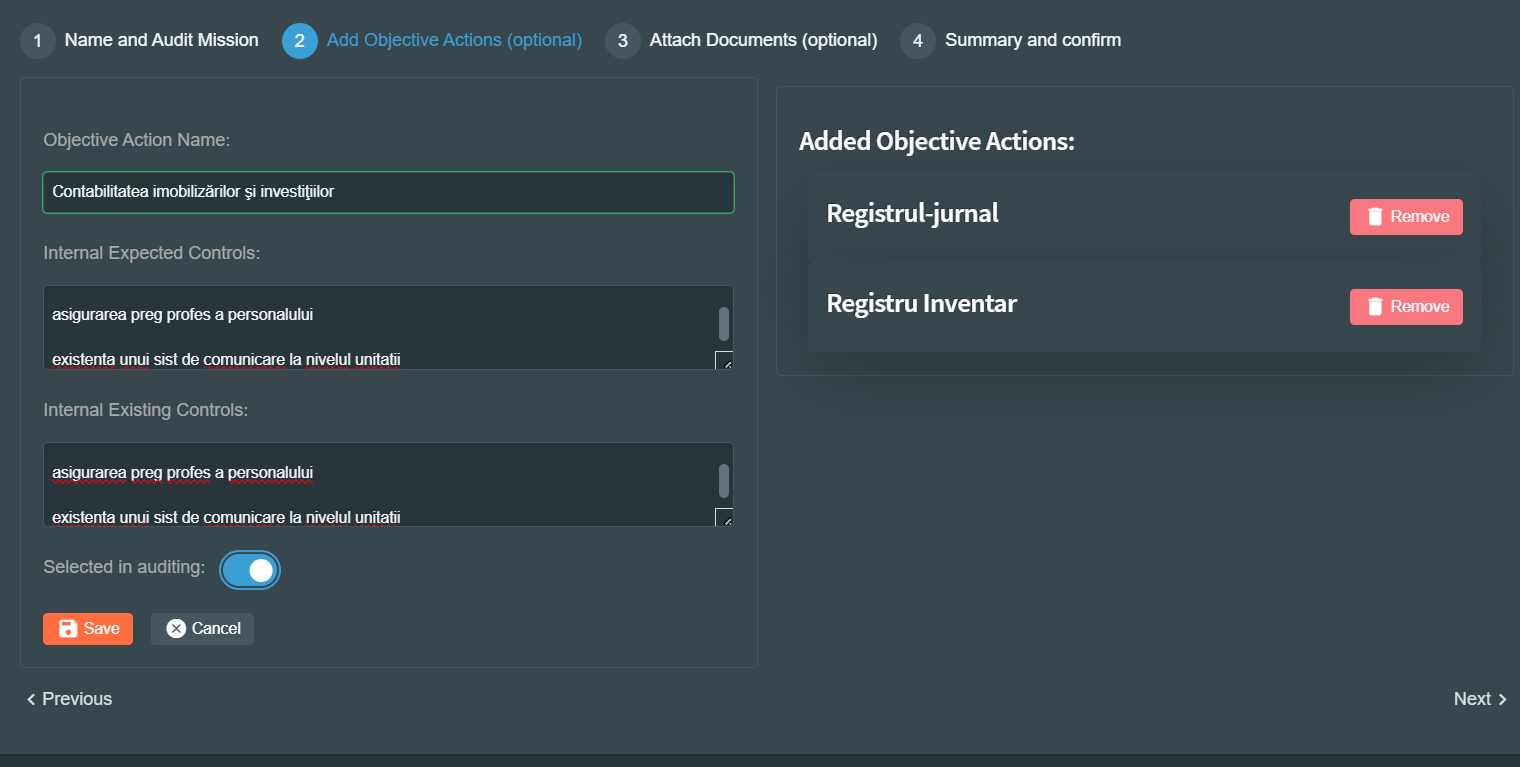
\includegraphics[width=0.9\textwidth]{c1/creare_obiectiv}
	\caption{Atasarea actiunilor specifice unui obiectiv}
\end{figure}

\subsection{Vizualizarea si accesarea ricurilor din misiuni anterioare}
Stabilirea obiectivelor de auditat, fiind un pas relativ important in procesul de audit public, o identificare cat mai precisa si corecta a riscurilor actiunilor acestora este cruciala pentu o buna desfasurare dar si pentru rezultate optime ale misiunii de audit.\\
Aplicatia ofera auditorului acces la un istoric de misiuni de audit public, in care acesta poate filtra doar misiunile de audit asupra departamentului la care se desfasoara si misiunea de audit curenta, astfel avand posibilitatea de analiza a riscurilor ce deja au fost descoperite, ajutandu-l 
astfel pe acesta sa stabileasca noi riscuri relevante, corecte si in conformitate cu situatia actuala.

\subsection{Identificarea si evaluarea riscurilor}
Platforma AudIT pune la dispozitia utilizatorului un mecanism de stabilire a riscurilor, acestia avand posibilitatea de a atasa noi riscuri identificate la o actiune, de a edita valorile riscurilor deja prezente sau de a sterge un risc din tabel in cazul in care acesta nu mai este conform sau o greseala in definirea acestuia a fost depistata.

Aceasta functionalitate este implementata prin intermediul unui tabel paginat, fiecare linie afisand informatii relevante despre risc, cum ar fi probabilitatea, impactul, scorul final (riscul propriu zis) dar si o scurta descriere a acestuia.

\vspace{1cm}
\begin{figure}[h]
	\centering
	
	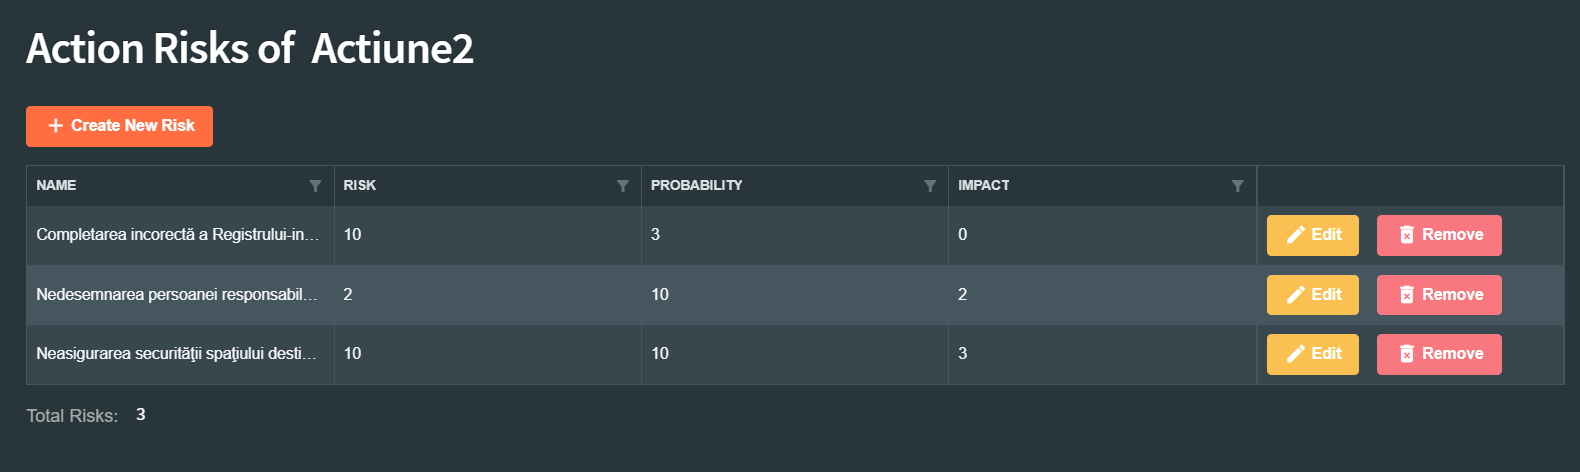
\includegraphics[width=0.9\textwidth]{c1/tabel_riscuri}
	\caption{Informatii sumare despre riscurile}
\end{figure}

De asemenea, in partea de jos a tabelului este afisat si numarul total de riscuri atasate actiunii respective, cat si scorul total al tuturor riscurilor, scor care il va ajuta ulterior pe auditor in stabilirea selectarii sau nu a obiectivul in auditare.

\subsection{Vizualizarea obiectivelor}

Ulterior crearii unui nou obiectiv al misiunii de audit, utilizatorul este redirectionat catre o pagina in care acesta poate viziona prin intermediul unui tabel toate obiectivele deja stabilite pentru misiunea respectiva de audit intr-un format cat mai intuitiv, usor de folosit si inteles .

Auditorul poate vizualiza toate actiunile specifice obiectivului pe care il analizeaza, avand in plus si informatii asupra numelui, data ulitimii modificari/accesari a acesteia, daca este selectat sau nu in procesul de auditare sau optiunea de a inspecta toate riscurile identificate pana la momentul curent, prin apasarea butonului 'More details' din dreptul coloanei 'Action Risks Details'.

\vspace{1cm}
\begin{figure}[h]
	\centering
	
	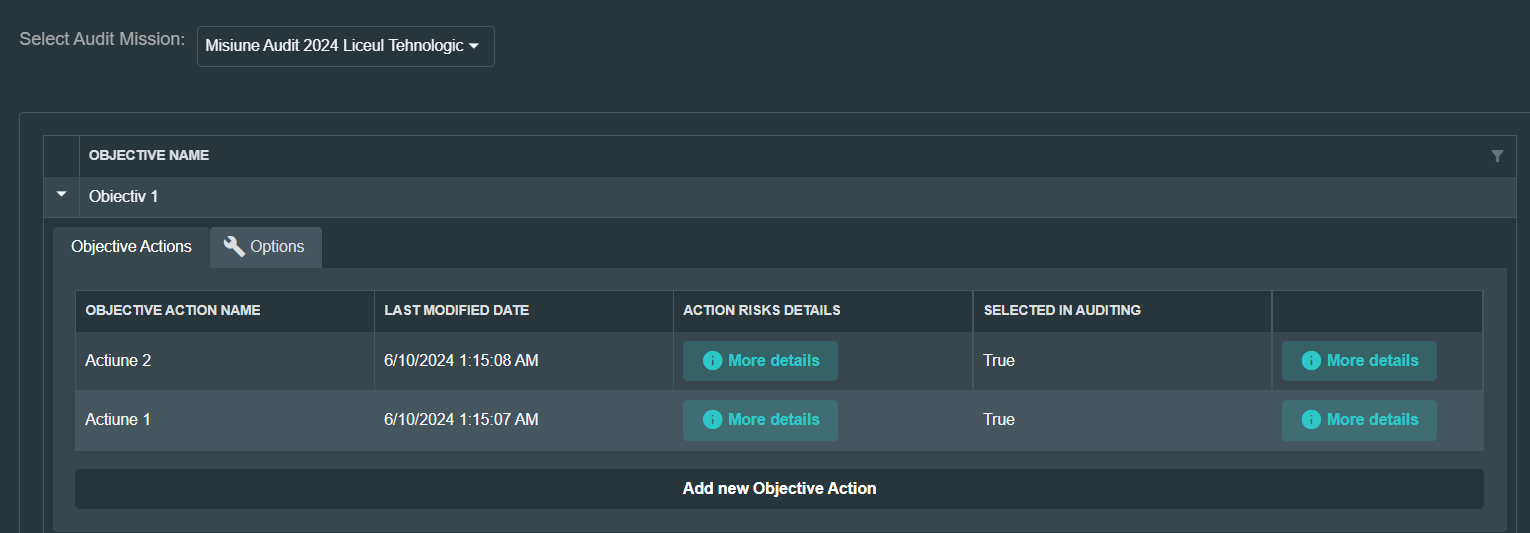
\includegraphics[width=1\textwidth]{c1/tabel_obiective}
	\caption{Informatii despre obiectivele misiunii de audit}
\end{figure}



De asemenea, utilizatorul poate naviga prin apasarea butonului 'More details' din dreptul ultimii coloane catre pagina dedicata detaliilor actiunii, in care acesta poate gasi mai multe amanunte referitoare la actiunea selectata.


\vspace{1cm}
\begin{figure}[h]
	\centering
	
	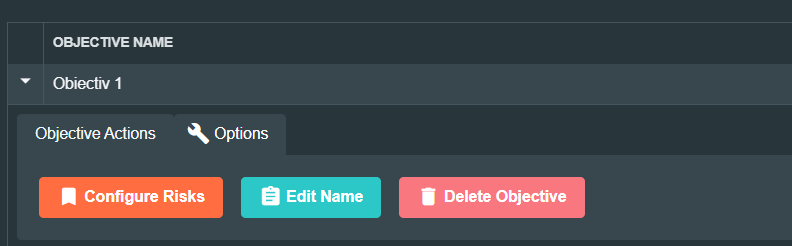
\includegraphics[width=0.9\textwidth]{c1/optiuni_suplimentare}
	\caption{Optiuni suplimentare gestionare obiectiv}
\end{figure}


\subsection{Pagina detalii actiune}
Pagina ofera auditorului o imagine de ansamblu asupra actiunii selectate, astfel acesta poate accesa si vizualiza detalii despre actiune cum ar fi:\\
\begin{itemize}
	\item un scurt rezumat al acesteia care contine numele, daca este sau nu selectata in procesul de audit, o lista de Controale Interne Asteptate respectiv o lista de Controale Interne Existente;
	
	\item  un tabel in care sunt afisate intr-un mod paginat riscurile asociate cu actiunea respectiva, afisand informatii despre impact,probabilitate si scorul riscului;
	
	\item  un tabel care contine informatii despre diferite FIAP-uri (Fisa de Identificare si Analiza a Problemei) care sunt asociate cu actiunea, afisand informatii despre numele FIAP-ului, perioada de start si de sfarsit a interactiunii, problema, cauza si recomandarea oferita de auditor;
	
	\item  un tabel  in care sunt afisate activitatile desfasurate de auditor avand ca motiv actiunea detaliata pe pagina, tabelul prezentand informatii despre numele activitatii, numele departamenutului asupra caruia a avut loc dar si tipul actiunii;
	
\end{itemize}


\vspace{1cm}
\begin{figure}[h]
	\centering
	
	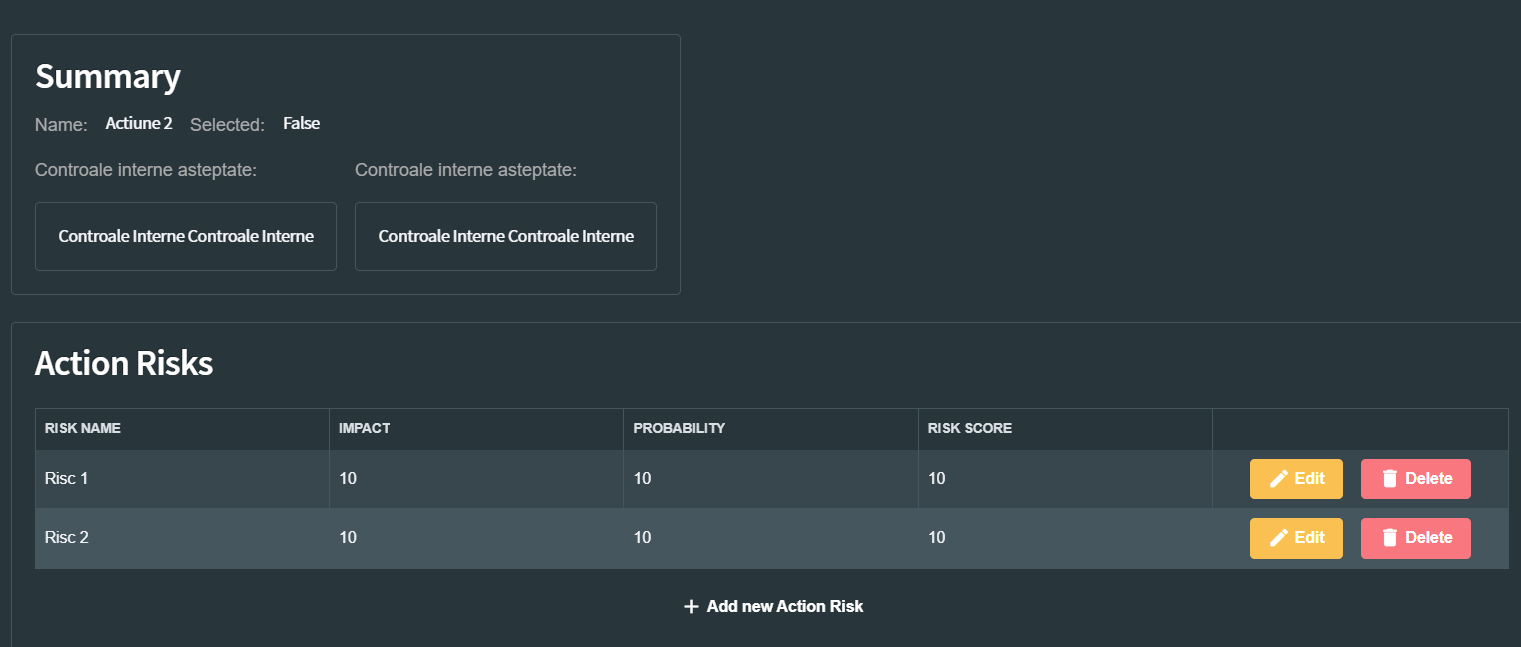
\includegraphics[width=0.9\textwidth]{c1/obiectiv_summary}
	\caption{Informatii despre obiectivul selectat}
\end{figure}


De asemenea, in partea de jos a fiecarui tabel, utilzatorul are optiunea de a adauga o noua entitate prin apasarea butonului 'Add new'.La apasarea acestuia, se deschide un dialog de tip 
form in care utilizatorul poate completa campurile pentru a initializa o noua intrare in tabel.

\vspace{1cm}
\begin{figure}[h]
	\centering
	
	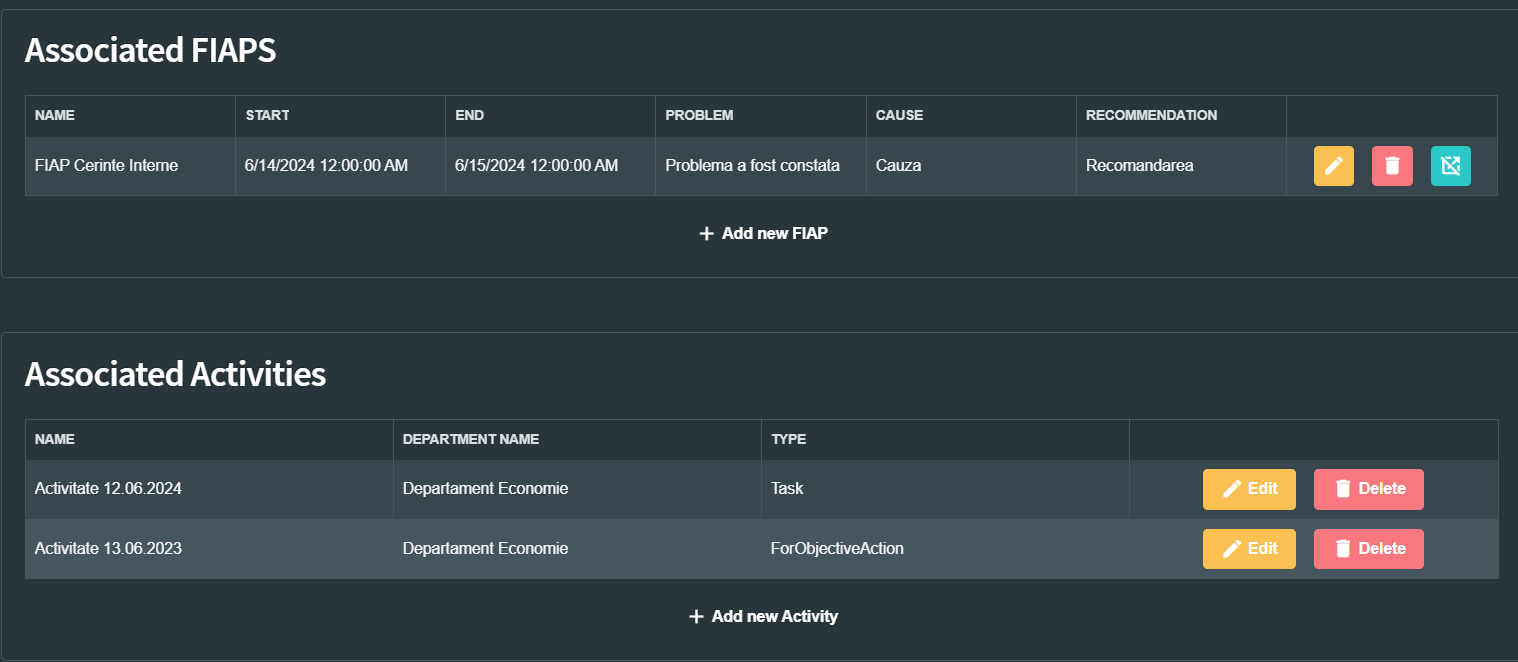
\includegraphics[width=0.9\textwidth]{c1/obiectiv_summary2.png}
	\caption{Informatii FIAP si Activitati}
\end{figure}


\subsection{Salvarea documentelor necesare pe platforma}

Inventarierea si accesarea documentelor necesare pentru desfasurarea unei misiuni de audit public este o etapa esentiala pentru asigurarea transparentei si eficientei procesului de audit public.

Platforma AudIT ofera aceste functionalitati utilizatorilor acesteia, astfel incat atat un auditor cat si membri ai departamentelor auditate care au acces la misiunea de audit, sa poata incarca si salveze pe platforma orice tip de document ce nu depaseste o anumita marime in dimensiune prestabilita.

La incarcarea unui astfel de document, auditorul are posibilitatea de a alege intre tipul documentului incarcat: document standard(un fisier de sine statator deja completat) sau document sablon(un fisier care necesita completarea acestuia inainte sau ulterior salvarii acestuia pe platforma).






 \subsection{Accesarea documentelor necesare pe platforma}
 
 Dupa crearea unui document si salvarea acestuia pe platforma, utilizatorii au optiunea de a vizualiza documentele elaborate de acestia respectiv cele la care li s-a oferit accesul.
 
 Afisarea documentelor se face prin intermediul unui tabel, unde sunt afisate informatii cum ar fi: numele documentului, tipul documentului, misiunea de audit de care apartine, starea in care acesta se afla, ultima data la care acesta a fost modificat si numele departamentului caruia ii este adresat (in cazul documentelor sablon).
 
 De asemenea, intrarile din tabel pot fi filtrate si sortate dupa diferite criterii, spre exemplu : alfabetic dupa numele sau tipul documentului, dupa starea in care acesta se afla sau dupa numele misiunii de audit de care acesta apartine.\\
 
 ---
 
 
 
 
  PIC HERE---\\
 
 
 \subsection{Completarea documentelor tip sablon}
 
	Una dintre sarcinile de baza ale auditorului, dar si un punct nevralgic al sistemului de audit public despre care am discutat anterior, il constituie nevoie de a inventaria si de a completa numeroase documente de tip sablon. Avand in vedere faptul ca numarul acestor documente este uneori de ordinul zecilor intr-o misiune de audit, o functionalitate care ar permite auditorului sa completeze in mediul digital acest tip de documente ar fi bine venita.
	
	Platforma AudIT ofera posibilitatea utilizatorilor sa completeze si sa editeze direct in aplicatie documentele de tip sablon salvate de acestia. Functionalitatea este implementata prin utilizarea unui simplu 
	MarkDown editor, in care documentul sablon este incarcat, editat, iar la finalizarea procesului, schimbarile facute sunt salvate.
	
	\subsection{Bara de navigare}
	Pentru facilitarea unui acces cat mai usor la principalele functionalitati ale platformei, utilizatorul se poate folosi de bara de navigare prezenta intotdeauna in partea stanga a aplicatiei.
	
	Aceasta este impartita in sectiuni specifice fiecarei entitati, astfel incat mentionam:
	\begin{itemize}
		\item  sectiunea misiunilor de audit unde regasim optiunea de a crea o noua misiune de audit, de a naviga la misiunea de audit selectata curent, vizualiza lista de misiuni de audit dar si o optiune de a cauta in fuctie de numele misiunii de audit; 
		
		\item sectiunea obiectivelor in care exista optiunile de creare a unui nou obiectiv, navigare catre pagina tututor obiectivelor, crearea a noi actiuni specifice unui obiectiv dar si posibilitatea de a cauta un obiectiv al misiunii de audit curente in functie de numele acestuia;
		
		\item sectiunea recomandarilor unde auditorul poate adauga o noua recomandare dar si vizualiza recomandarile deja existente;
		
		\item sectiunea documentelor unde similar, merg adaugate noi documente si vizualiza documente deja existente pe platforma;
		
		\item sectiunea activitatilor unde utilizatorul poate consemna activitati noi desfasurate sau naviga spre cele existente deja;
		
		\item sectiunea dedicata exportarii, unde auditorul poate naviga spre diferite pagini de convertire a obiectivelor, actiunilor si a riscurilor in diferite formate dar si autocompletare a unor documente oficiale de tip sablon, cum ar fi Fise de Identificare a Problemei sau Raport de Evaluarea a Riscurilor;
		
		\item sectiunea de control al accesului, unde auditorul sau reprezentantii institutiilor audidate pot consulta resursele la care au acces de scriere sau citire respectiv a oferi acces altor utilizatori la resurse personale;
		
		\item sectiunea de configurare, unde un utilizator cu drepturi elevate poate configura institutiile respectiv departamentele inregistrate pe platforma, adaugand, editand sau eliminand instante dintre acestea.
		
		
		
		

	\end{itemize}
\newpage
   De asemenea, bara de navigare se actualizeaza in functie de statusul de autentificare si rolul pe care utilizatorul il are.
   \begin{figure}[h]
   	\centering
   	\begin{minipage}{.5\textwidth}
   		\centering
   		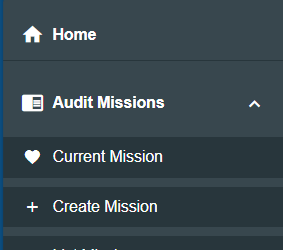
\includegraphics[width=.9\linewidth]{c1/navbar_logat}
   		\caption{Utilizator autentificat}
   		
   	\end{minipage}%
   	\begin{minipage}{.5\textwidth}
   		\centering
   		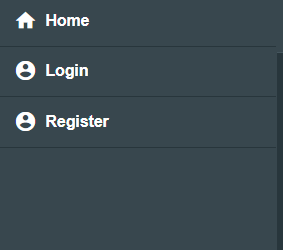
\includegraphics[width=.9\linewidth]{c1/navbar_nelogat.png}
   		\caption{Utilizator neautentificat}
   		
   	\end{minipage}
   	
   	
   \end{figure}

	\subsection{Gestionarea accesului la resurse partajate}
	
	 O componenta cheie in desfasurarea corecta a unei misiuni de audit este colaborarea intre partile participante la misiunea de audit.
	 
		Functionalitatea de acordare a accesului la resurse, contribuie la o colaborare cat mai stransa intre membrii partipanti la misiunea de audit, astfel un auditor poate acorda acces de scriere sau citire la diferite resurse create de acesta.
		
		In plus, o lista completa a accesului primit sau oferit se poate vizualiza de catre utilizator pe o pagina dedicata, unde sub forma unui tabel sunt prezentate informatii specifice cum ar fi numele si tipul resursei si email-ul utilizatorului caruia i s-a oferit  acces
		
	\subsection{Gestionarea activitatilor desfasurate}
	 Prin aceasta functionalitate, auditorul poate consemna orice sarcina pe care acesta o efectueaza pe platforma prin intermediul unei activitati. Aceasta cuprinde informatii referitoare la actiunea asupra careia s-a efectuat o activitate, departamentul asociat dar si tipul activitatii care poate fi asociat unei misiuni, unei actiuni sau pur si simplu o sarcina administrativa.
	 
	 De asemenea , toate activitatile consemnate intr-o misiune de audit, pot fi vizualizate de catre auditor intr-o pagina dedicata, acestea fiind afisate prin intermediul unui tabel care ofera informatii referitoare la numele acesteia, tipul actiunii sau departamentul asupra cauia s-a realizat respectiva sarcina.
	 
	
	\subsection{Profilul personal}
	Pagina profilul personal este locul unde utilizatorul poate sa isi verifice informatiile personale care sunt disponibile pe platforma avand posibilitatea de a le edita. Informatiile cuprind detalii de contact, cum ar fi adresa de email, numar de telefon al institutiei, numar de telefon personal, adresa fizica de contact respectiv daca acesta este verificat sau nu.
 
	
	\subsection{Sistemul de notificari}
		Functionalitatea permite vizualirea notificarilor in ceea ce priveste crearea de noi resurse, primirea accesului la o anumite resursa sau notificari in ceea ce priveste actualizarea sau implementarea unor solutii la recomandarile impuse de auditor din partea reprezentantilor institutiei asupra careia are loc misiunea de audit.


	\section{Solutii similare}
	Solutia descrisa nu este o idee unica, dar este esential sa studiem si sa intelegem modul in care solutiile similare abordat aceasta problema, avand astfel posibiliatea sa identificam puncte forte cat si puncte slabe ale aplicatiei ce merg ulterior imbunatatite, inovand acolo unde este posibil.
	
	In sectiunea urmatoare o sa fie prezentate cateva solutii similare adresate problemei de digitalizare in domeniul auditului public si o sa fie analizate functionalitatile forte ale acestora. 
	
	\subsection*{Audit Pro}
	
	Audit Pro este o aplicatie dezvoltata in special pentru sistemul de operare Windows si care incearca sa ofere un mediu de lucru doar auditorilor din institutiile publice.\\
	Solutia oferita este una care se bazeaza pe achizitionarea acesteia contra unui pret, oferid in pachet si o configurare initiala a institutiilor si membrilor din departamentul de audit.
	
	Aceasta ofera functionalitati similare cu solutia descrisa in acest document, dar printre care se evidentiaza: 
	\begin{itemize}
		\item accesul la un calendar unde auditorul poate vizualiza evenimentele importante ce vor avea sau au avut loc, avand de asemenea posibilitatea de a adauga noi evenimente in acesta;
		
		\item o pagina dedicata analizei costurilor desfasurarii anumitor activitati specifice unei misiuni de audit: costuri de deplasare, diurne etc;
		
		\item un meniu de ajutor unde utilizatorul poate accesa informatii ajutatoare in vederea utilizarii anumitor functionalitati din aplicatie;
		
	\end{itemize}
	
	\vspace{1cm}
	\begin{figure}[h]
		\centering
		
		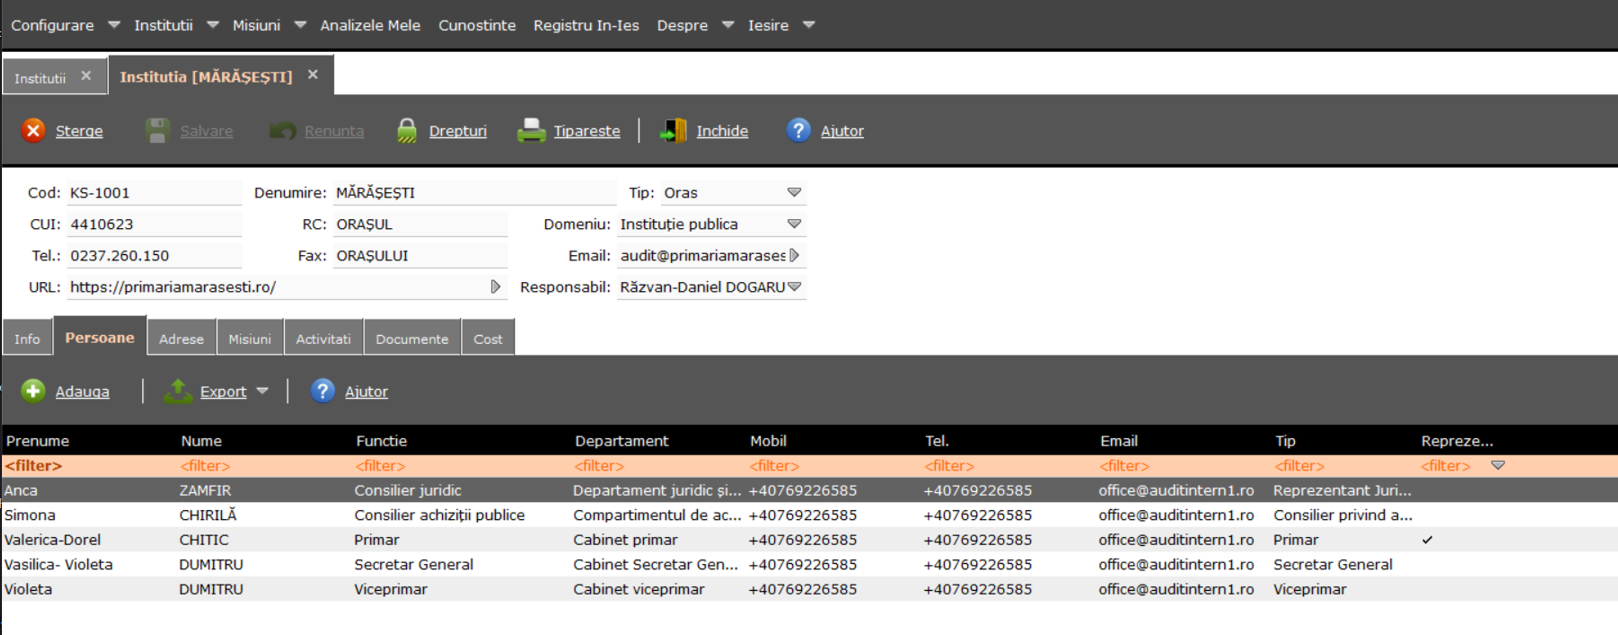
\includegraphics[width=0.9\textwidth]{c1/auditpro1}
		\caption{Tabel din aplicatia Audit Pro}
	\end{figure}
	
	
	
Pe de alta parte, solutia descrisa prezinta si anumite dezavantaje care constau in modul in care aceasta a fost implementata, unul dintre acestea fiind limitarea strict la utilizarea acesteia numai pe sistemul de operare Windows, marginind in acest mod alte sisteme de operare prezente.
De asemenea, din punctul meu de vedere, aspectul grafic si interfata pe care aceasta solutie o prezinta nu este una foarte intuitiva si poate induce in eroare utilizatorii in anumite situatii.
\vspace{1cm}
\begin{figure}[h]
	\centering
	
	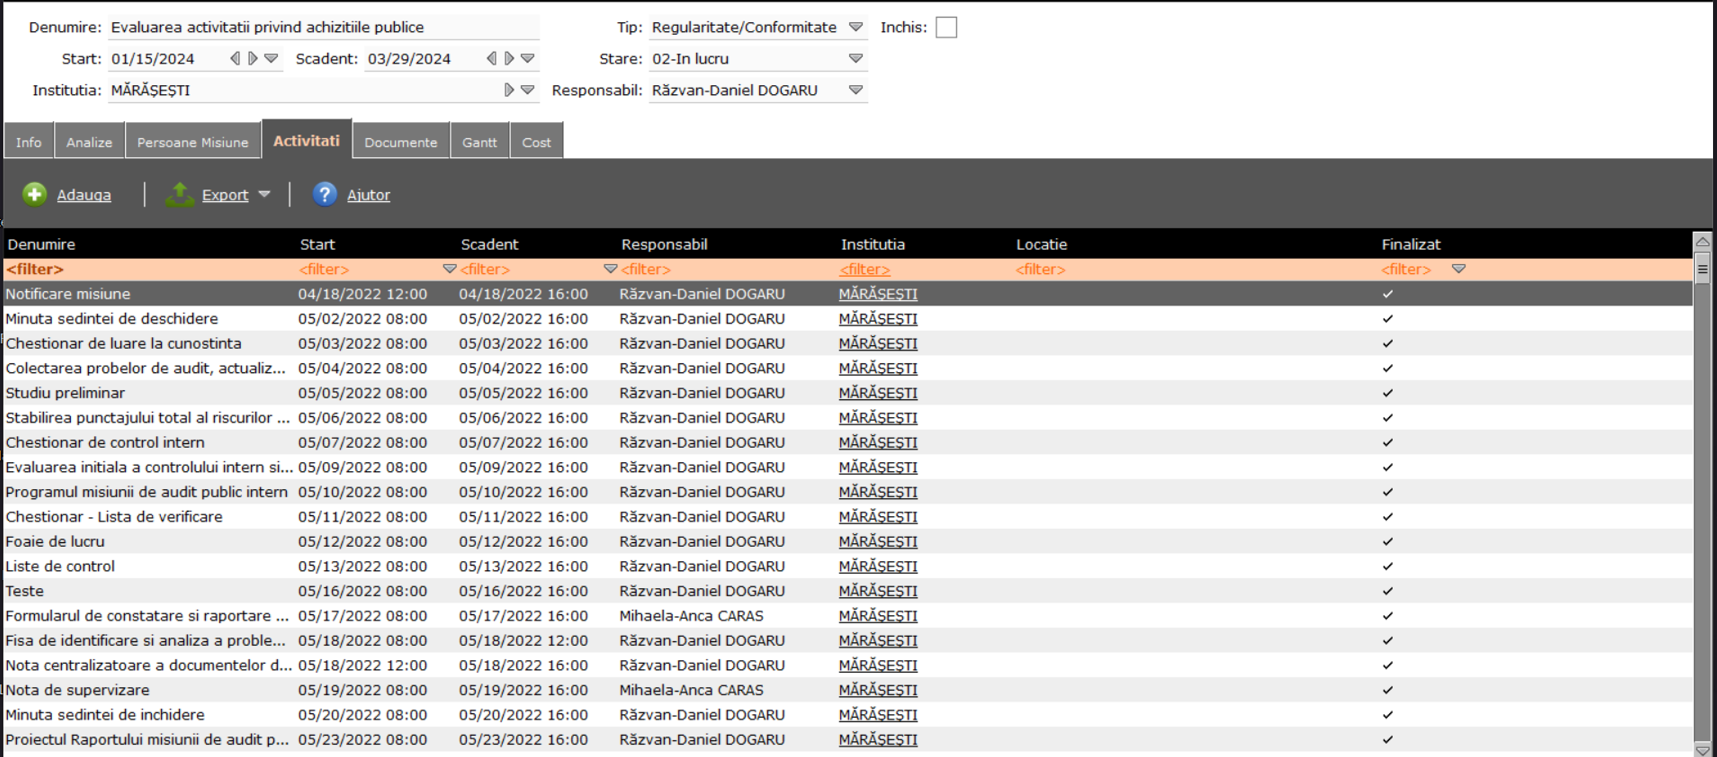
\includegraphics[width=0.9\textwidth]{c1/auditpro2}
	\caption{Tabel din aplicatia Audit Pro}
\end{figure}

	\newpage
	\subsection*{Site Audit Pro }
	
	Chiar daca numele este similar cu solutia prezentat similar, este vorba despre un alt proiect, de aceasta data o platforma web cu suport si pentru aplicatie mobila care prezinta solutii pentru auditul in sectorul privat, cel al companiilor.
	Din informatiile prezente pe pagina  lor de prezentare, se poate trage concluzia ca aceasta solutie este una ajunsa la maturitate, primind constant actualizari in ceea ce priveste functionalitatile oferite de aceasta.
	 
	Dintre numeroasele facilitati pe care aceasta solutie le ofera, cele mai importante si cu un impact mai mare ar putea fi:
	\begin{itemize}
		\item posibilitatea de a lucra in mediul \textit{offline} pe platforma mobila, informatiile fiind actualizate cu server-ul principal in momentul in care exista o conexiune la internet;
		
		\item sincronizarea proiectelor pe toate dispozitivele (Web, Android si IOS) astfel incat toate informatiile sa fie actualiate in timp real;
		
		\item organizarea proiectelor si resurselor in directoare, facilitand astfel o navigare mai eficienta ;
	\end{itemize}
	\begin{figure}[h]
		\centering
		
		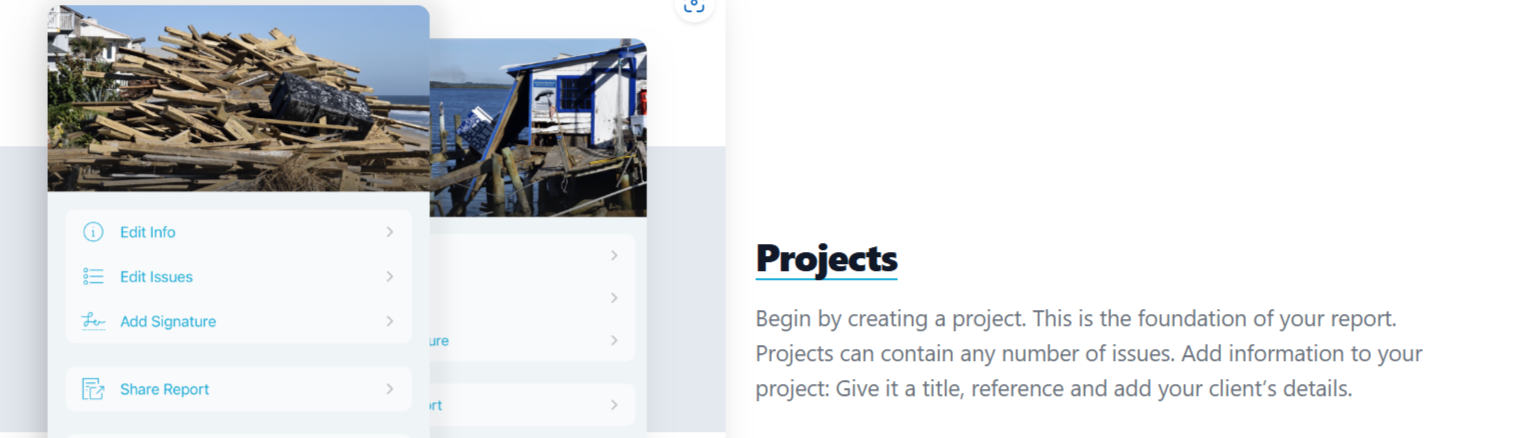
\includegraphics[width=0.6\textwidth]{c1/auditpro3}
		\caption{Tabel din platforma Site Audit Pro}
	\end{figure}
	
	Cu toate acestea, un dezavantaj pe care aceasta solutie il ofera este acela ca procedurile pe care acesta este construit, nu se muleaza si nu corespund in cea mai mare parte cu cele din sistemul de audit public din Romania, utilizatorii trebuind astfel sa se adapteze si sa incerce pe cat posibil sa personalizeze si sa modifice functionalitatile oferite de acestia.
	
	
	
	
